
\begin{figure}
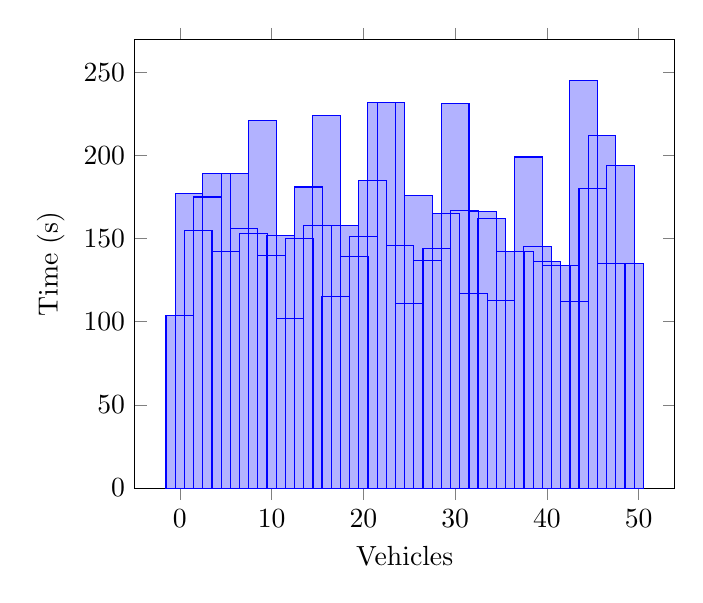
\begin{tikzpicture}
\begin{axis}[
legend style={anchor=west},
xlabel=Vehicles,
ylabel=Time (s),
ymin=0,
ybar,
]
\addplot coordinates {
(0, 104)
(1, 177)
(2, 155)
(3, 175)
(4, 189)
(5, 142)
(6, 189)
(7, 156)
(8, 153)
(9, 221)
(10, 140)
(11, 152)
(12, 102)
(13, 150)
(14, 181)
(15, 158)
(16, 224)
(17, 115)
(18, 158)
(19, 139)
(20, 151)
(21, 185)
(22, 232)
(23, 232)
(24, 146)
(25, 111)
(26, 176)
(27, 137)
(28, 144)
(29, 165)
(30, 231)
(31, 167)
(32, 117)
(33, 166)
(34, 162)
(35, 113)
(36, 142)
(37, 142)
(38, 199)
(39, 145)
(40, 136)
(41, 134)
(42, 134)
(43, 112)
(44, 245)
(45, 180)
(46, 212)
(47, 135)
(48, 194)
(49, 135)
};

\end{axis}
\end{tikzpicture}
\label{tik:100:52}
\caption{100 percent diving with GSC on route $52$}
\end{figure}
